\subsection{How to search for new phenomena?} \label{sec:stat1} 
%\subsection{What is a search?}
In experimental physiscs  an observation of a new phenomena or its exclusion  is 
carachterized by means of statistical statements, in this sense one can say that statistic is the language 
of experimental physics.
Search for new physics at the LHC extesively uses frequentistic statistical tests~\cite{LHCstat}.
%to make
%robust statements about the exsistence or the exclusion of new phenomena, %to make robust statements... qualcosa qui
In this section an itroduction to statistical tests is given, for more details see section~\ref{sec:result}.
 
A \emph{statistical test} is a rule to reject or accept an hypotesis, where for hypotesis is meant 
a statement about the distribution of the data. Typically new physics searches are looking for a signal 
that is additive on top of the background, is then natural to compare two hypotesis:
the background only hypotesis $H_{0}$, or null hypotesis, and the signal plus background hypotesis $H_{1}$, which is the alternative.
In the process of decision making is common to define what is called a \emph{signal region} (SR), which is simply
a set of selections applied to data aimed to enhance signal with respect to the background, 
the observed number of events in the SR, $N_{SR}$,  are used to make probabilistic statements about the two hypotesis.
$N_{SR}$  is in fact a random
variable described by a Poisson distribution, where, in case the null hypotesis is true, $\nu_{B}$ events are expected, otherwise 
in case $H_1$ is true $\nu_{B} + \nu_{S}$ events are expected. The two probability distributions for the two hypotesis
totaly describes the \emph{probability model} for this counting experiment.
%
%the probability model for null and the alternate hypotesis is then respectively 
%$\text{Pois}(N_{SR}|\nu_{B})$ and $\text{Pois}(N_{SR}|\nu_{B} + \nu_{S})$.
Is clear then that the evidence for a signal shows up as an excess of 
events, a way to quantify the conpatibility of the null hypotesis with data
is to make a \emph{significance} test: calculate the probability that 
the background-only would produce at least as many
as the observed events, which is the so called of p-value and in this case is expressed by the formula:
$$
\text{p-value} = \sum_{n=N_{SR}}^{\infty} \text{Pois}(n|\nu_{B})
$$
Calculating  p-values is a way to characterize an excess, in high energy physics the commonly accepted p-value that is
qualified as a discovery is $2.87 \times 10^{-7}$, which is an extremely low probability for the null hypotesis to be true
and corresponds to five standard deviation for a gaussian distribution. 

In case no excess is observed, the procedure is to build a statisctical test where the 
null hypotesis is accepted and at the same time the signal hypotesis
is rejected with a fixed predetermined probability, called confidence level.
A statistical test is a rule that defines a region in the space of data for which
a given hypotesis can be accepted or rejected, often rather than using a full set 
of data $\mathcal{D}$, it is convenient to define a \emph{test statistic}, T, which is usually a single
number computed from the data, the two hypotesis implies different distributions for T, 
then one defines an acceptance region \emph{W} in terms of the test statistic, if 
$T \in W$ the $H_{0}$ is rejected, $H_{1}$ accepted and vice versa,
the probability with which one rejects $H_{1}$ or $H_{0}$ is then given by the choice of
\emph{W} and T. Neuman and Pearson provided a framework for hypotesis testing that addresses the 
choice of the test statistic \cite{NP}.
%such that 
%$P(T \in W | H_{0}) \leq \alpha$, where $\apha$ is the size of the test and correspond to the probability
%for which $H_{0}$ is rejected when is true, 

A discriminating variable is often used to help separating signal and backgrounds, this can be any of the observables of
the experiment, a usually chosen observable is for example the invariant mass of the final state particles. The expected
distributions of this observable for the two hypotesis completes the above
mentioned probability model, the actual implementation is achieved by means of an histograms, 
i.e. by discretizing the distribution of the observable and making a counting experiment
for each bin of the histogram, the resulting probability model is then a product of Poissons: 
\begin{equation}\label{markedpoisson}
\prod_i \text{Pois}(n_i^{observed} ~ | ~ s_i(\vec{\theta}) + b_i(\vec{\theta})) 
\end{equation}
where $s_i$ and $b_i$ are  the number of expected signal and background events in the bin $i$, while $n_i$ are the
actual observed events in the bin $i$. Here is made explicit that the signal and backgrounds expectations
depends also on a set of additional parameter $\vec{\theta}$, called \emph{nuissance parameters}, 
those embed effects like detector mismodeling and theoretical uncertainty.

%A statistical test is a rule that define a region in parameter space for which  a given hypotesis can be accepted or rejected.
%Often rather than using a full set of data $\vec{X}$, it is convenient to define a \emph{test statistic}, t, which is usually a single
%number, it is a quantity calculated out of the data, a mapping of a set of measurements into a single number. The test statistic, that is usually
%connected to the discriminating variable, would then have a different distribution for the different hypotesis, one can then define $\alpha$
%called the size of the test and $t_{\alpha}$ for which $P(t < t_{\alpha} | H_{0}) \leq \alpha$ then in this case $H_{0}$ is rejected.

%- Alternative: NP provided a framework for hypotesis testing that addresses the choice of the test statistic. First one defines 
%an acceptance region in terms of a test statistic, such that if $T(\vec{X}) < t_{\alpha}$ one accepts the null hypotesis. 
%One can think of $T(\vec{X}) = t_{\alpha}$ as a counturn in the space of the data which is the boundary to this acceptance region.
%Then one defines the size of the test $\alpha$ which is the probability for the null hypotesis to be rejected when true,
%the test is totally asymmetric: if the null hypotesis is rejected then the alternate is accepted (is this true??)....

Summarizing, there are several ingredients that constitute a search for new physics:
\begin{itemize}
	\item Definition of a signal region in data where signal is enhanced with respect to the backgrounds, detailed for this analysis in section \ref{sec:topology} 
	and \ref{sec:selectiona}.
	\item Definition of a discriminating variable which is usefull to disentangle between signal and backgrounds, see section \ref{sec:mmc}.
	\item Definition of the probability model, i.e., the expectation for the distribution of the discriminating variable
		 for signal and background hypotesis, this is one of the most importat
		point of a search and main part of the work of this thesis, detailed in section \ref{sec:BackgroundEstimation}.
	\item Definition of a test statistics to quantify an observation or an exclusion, which is discussed for the LHC in section \ref{sec:result}.
\end{itemize}

\section{limits}

As its has allready been outlined in section~\ref{sec:stat1}, any statistical test is based on probability
distribution, once a probability density function (p.d.f.) is defined, one can calculate its value for a given 
set of data obtaining what is called a "likelihood".  Taking the marked Poisson
p.d.f. in equation~\eqref{markedpoisson}  one obtain the following likelihood function:
  

\begin{figure}[tp]
  \centering
 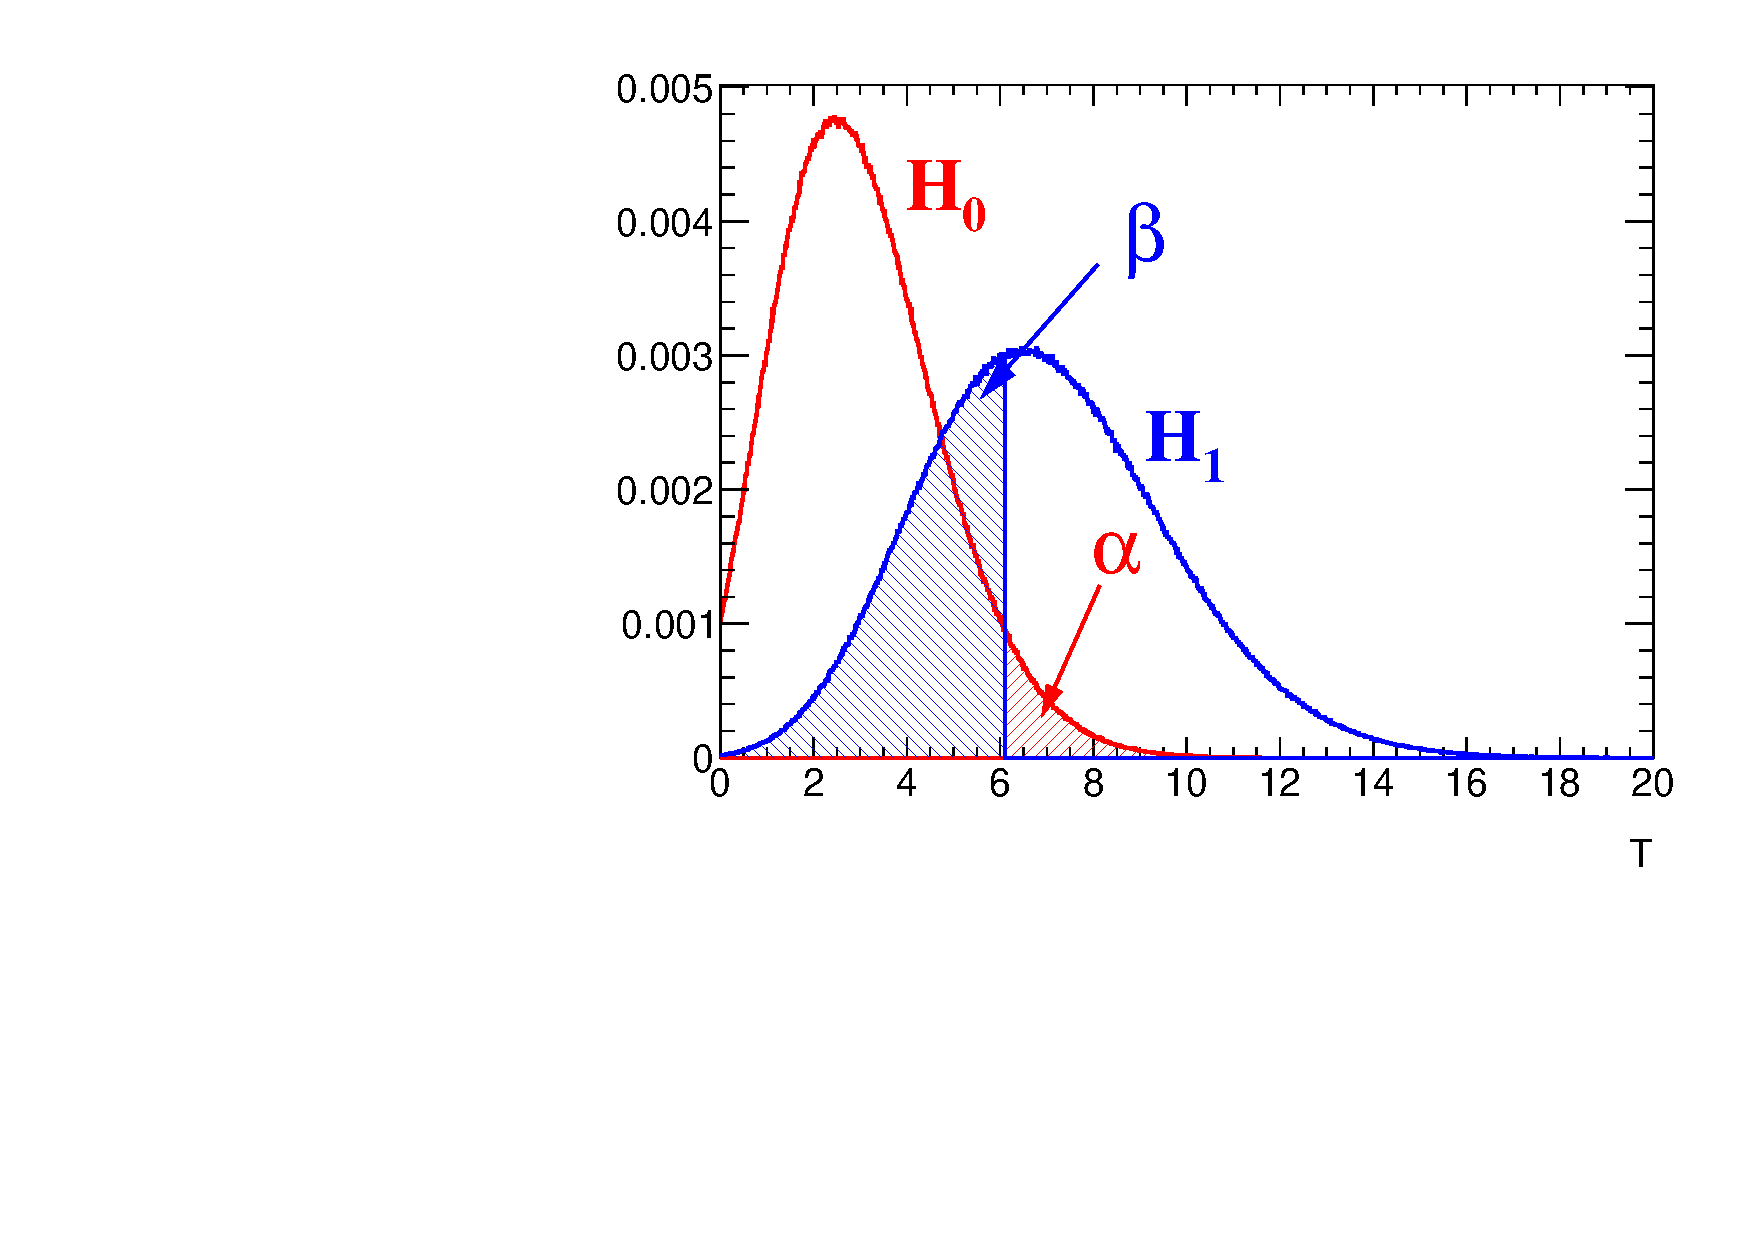
\includegraphics[width=0.5\textwidth]{figure/test_stat.pdf}
  \caption{Example of a test statistic which in this case is just the total number of events of a counting experiment.
	Under the hypotesis $H_0$ are expected four events, while under the $H_1$ seven  events are expected.} 
\label{fig:teststat}
\end{figure}

